\section{Related work} \label{sec:rel}
Named-entity recognition(NER) comprises two tasks. Retrieval of NE's is regarded as the primary task, and type classification of retrieved NE's as the secondary task \cite{buitinck2012two}. An averaged perceptron is used for both stages, each consisting of its own feature parameters. The benefit of two-staged NER, in which a different algorithm per stage is used, lies in the opportunity of optimizing each algorithm individually.  

Recently, the most prevalent implementations of NER apply a supervised machine learning approach \cite{desmet2014fine} \cite{buitinck2012two} \cite{graus2014semanticizing}. An annotated corpus is required for apprehension of features (for instance syntax and context) that indicate the occurrence of an NE, as well as the type. This is state of the art as opposed to handcrafted rules \cite{zhou2002named}. Rule-based systems, however, are not completely disregarded mainly "... due to the associated
transparency of the internal system state, which leads to better explainability of errors." \cite{chiticariu2010domain}. The downside of learning off an annotated corpus is the large training corpus that is required, along with domain resemblance to the goal domain of the NER application. Currently, the only Dutch corpus that was made publicly and freely available, is the CoNLL-2002 data set of news items that appeared in the Belgian newspaper \textit{De Morgen}. The data set contains 301,418 tokens with annotated Part-of-Speech(PoS) and IOB-tag\footnote{\url{https://en.wikipedia.org/wiki/Inside_Outside_Beginning}} hyphenated with entity type. IOB, short for inside-outside-beginning, is an indicator for a token to be interpreted as the beginning of an entity consisting of multiple tokens; second or one thereafter in the tag sequence; or outside, meaning not an entity on its own or part of one. When spoken of an \emph{entity tag} in this thesis, the complete tag (IOB+type) is referred to, which can be understood from the visualization in figure \ref{fig:iob}.

\begin{figure}
    \centering
    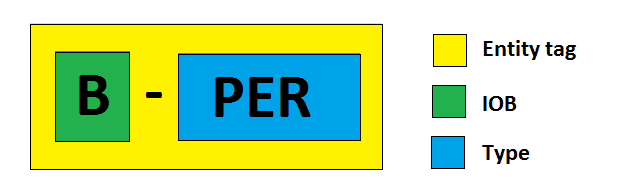
\includegraphics[scale=0.4]{fig/entity_tag}
    \caption{The components of the entity tag}
    \label{fig:iob}
\end{figure}

A variety of classifier types can be chosen from, such as a memory-based learning classifier, a support-vector machine or a conditional random field.
No significant results are achieved by a combination of different classifiers, subsequently classifying based on weighted votes, as is shown by an in-depth evaluation of an ensemble of classifiers for Dutch  \cite{desmet2014fine}. Higher precision and recall are found by the optimization of features in a single classifier.

Likewise an \emph{unsupervised} machine learning approach has been suggested, for which no manual construction of gazetteers or annotated corpora is required \cite{kazama2008inducing}. While gazetteers are considered the most precise for NER, maintaining large dictionaries can be expensive. Clustering of verb-multi-noun dependencies allows for the automatic formation of gazetteers, avoiding said issue.

Frog is an expansion to TADPOLE \cite{bosch2007efficient}. The system is modular, composed of tokenization, lemmatization, chunking and morphological segmentation of word tokens. In addition NE's are detected in Dutch texts using a memory-based tagger \cite{daelemans2010mbt}. Frog is designed for high accuracy, fast processing and low memory usage, qualifying itself to process numerous parliamentary items. Frog is trained on the SoNaR corpus \cite{oostdijk2008d} consisting of one million annotated and manually verified NER labels. The NER module has not been trained on PoS, but on the contextual relation between words and entity tags directly.  The assignment decision for each token is made with a lookup in memory, in which the instance base is stored. Unknown words are classified by a comparison to this instance base. The class of the instance that matches the contextual and internal features of the unknown instance the closest, is chosen. A processed Dutch sentence example is displayed in figure \ref{fig:frog_out}. Each token is associated with its own features, which are delimited by tabs.

\begin{figure}
    \centering
    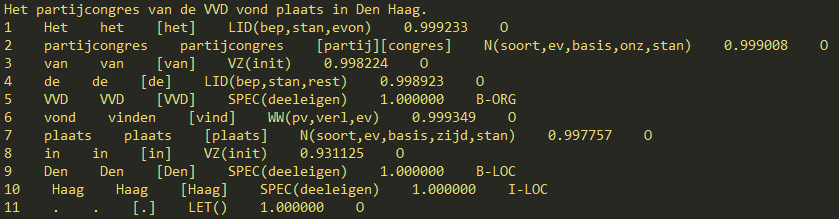
\includegraphics[scale=0.7]{fig/frog_output}
    \caption{The raw output of a processed Dutch sentence using Frog}
    \label{fig:frog_out}
\end{figure}





